\documentclass{beamer}

\usepackage{beamerthemesplit}
\usepackage{graphicx}
\usepackage{hyperref}
\DeclareGraphicsRule{*}{mps}{*}{}

\usetheme{Warsaw}
\setbeamercovered{transparent}
\colorlet{darkblue}{blue!80!black}
\colorlet{darkgreen}{green!80!black}
\newcommand{\xlink}[1]{\color{darkblue}{#1}}

\title{Constructing the TreeFam Database}
\author{Heng Li}
\institute[inst]{The Wellcome Trust Sanger Institute}
\date{March 16, 2007}

\begin{document}

\frame{\titlepage}

\AtBeginSection[]{\frame{\frametitle{Outline}\tableofcontents[current]}}
\part{Main Part}

\frame{\frametitle{Outline}\tableofcontents[part=1]}

\section{Introduction}
\subsection{Concepts and Background}
\frame {
	\frametitle{Species, sene and phylogeny}
	\begin{itemize}
	\item A \alert{species} is a group of organisms capable of interbreeding
		with each other but not with members of other species. (interbreeding separation)
	\item A \alert{gene} is a DNA segment that contributes to phynotype/function.
		In the absence of demonstrated function a gene may be characterized
		by sequence, transcription or homology.
	\item \alert{Phylogenetics} is the science of studying the evolutionary
		relationships (\alert{phylogenies}) of a group of organisms or genes.
	\end{itemize}
}
\frame {
	\frametitle{A species tree}
	\hypertarget{spec-tree}{}
	{\center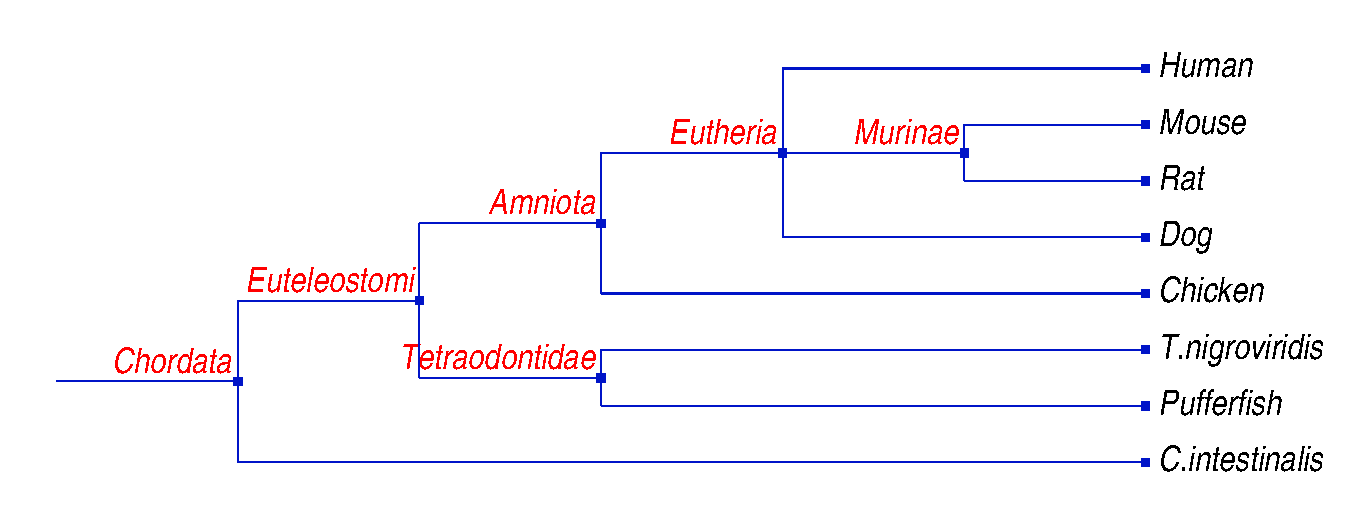
\includegraphics[width=\textwidth]{spec}}
	{\hyperlink{gene-tree}{\beamergotobutton{gene tree}}}
}
\frame {
	\frametitle{Gene families and orthologs}
	\begin{itemize}
		\item \alert{Gene family} is a group of gene that are descendant from a single gene.
		\item \alert{Homologs} are genes that are descendant from a signle gene.
		\item \alert{Orthologs} are genes in different species that originate from a single
			gene in the last common ancestor of these species.
		\item Homologs that are not orthologs are \alert{paralogs}.
	\end{itemize}
}
\frame {
	\frametitle{Interpretting the history of gene evolution}
	{\center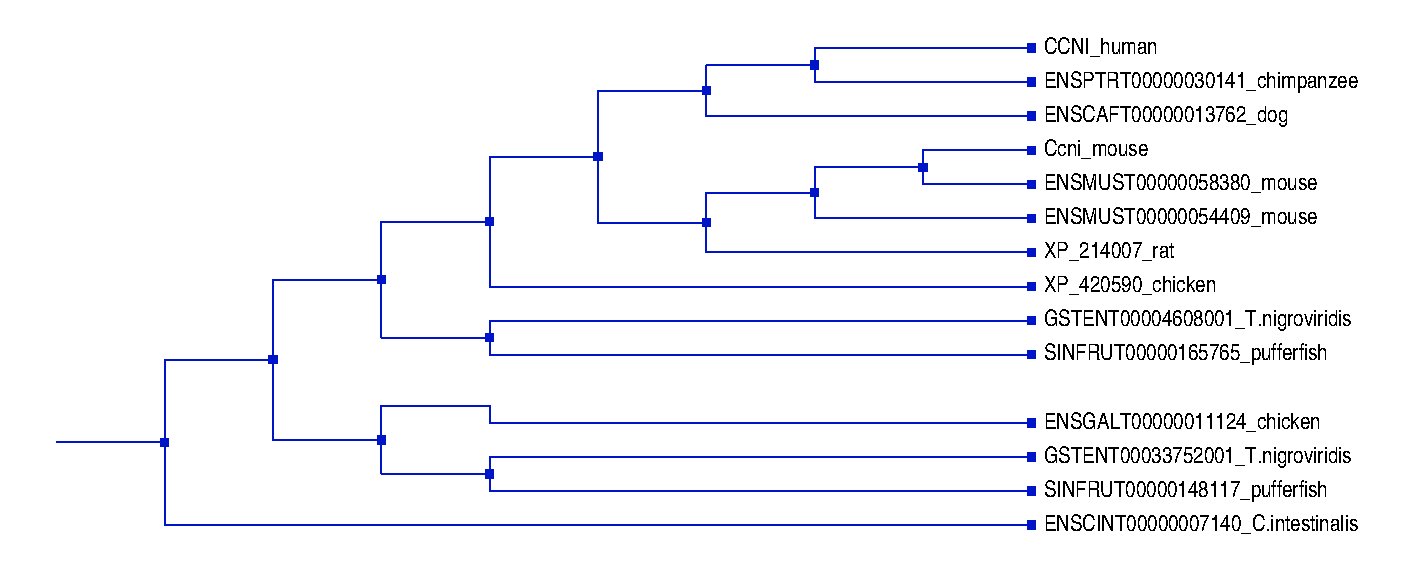
\includegraphics[width=\textwidth]{gtree-plain}}
	\begin{itemize}
	\item {\sf CCNI\_human} and {\sf XP\_420590\_chicken} are orthologs.
	\item {\sf CCNI\_human} and {\sf ENSGALT00000011124\_chicken} are paralogs.
		({\it See also} \hyperlink{spec-tree}{\beamergotobutton{species tree}})
	\end{itemize}
}
\frame {
	\frametitle{Interpretting the history of gene evolution}
	\hypertarget{gene-tree}{}
	{\center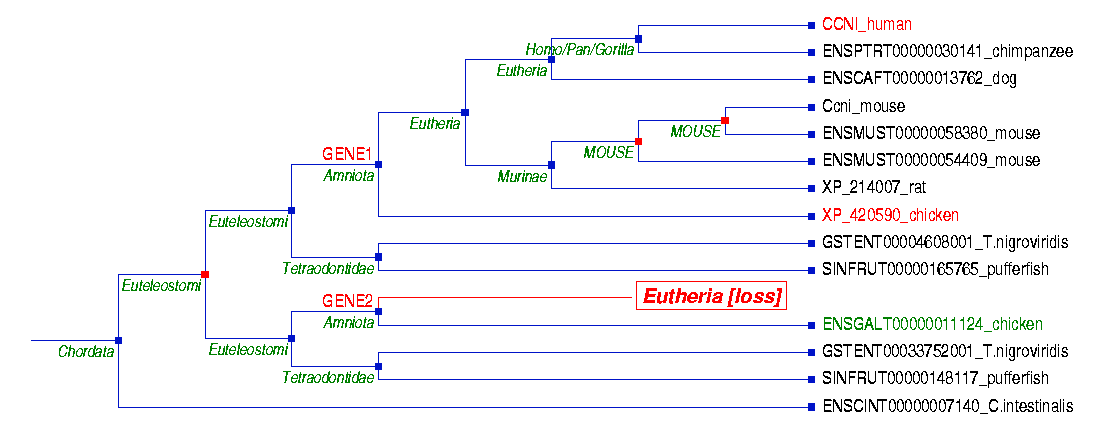
\includegraphics[width=\textwidth]{gtree}}
	\begin{itemize}
	\item {\sf CCNI\_human} and {\sf XP\_420590\_chicken} are orthologs.
	\item {\sf CCNI\_human} and {\sf ENSGALT00000011124\_chicken} are paralogs.
		({\it See also} \hyperlink{spec-tree}{\beamergotobutton{species tree}})
	\end{itemize}
}
\frame {
	\frametitle{Why is gene evolution important?}
	\begin{itemize}
	\item Transfer gene annotations across different species.
	\item Gene evolution is subjected to functional shifts and, in turn, reflects functional implication.
		\begin{itemize}
		\item Infer meaningful mutations.
		\item Detect pseudogenes and genes under positive selections.
		\item Reconstruct protein-protein interaction networks.
		\end{itemize}
	\item Pave the way for other related evolutionary studies.
		\begin{itemize}
		\item Intron evolution
		\item Genome-wide duplications
		\end{itemize}
	\end{itemize}
}
\subsection{What is TreeFam?}
\frame {
	\frametitle{What is TreeFam?}
	\begin{itemize}
	\item \alert{TreeFam} is a database of curated phylogenetic trees of animal gene families.
		\begin{itemize}
		\item A protein classification database: classify genes into families,
			and assign a name to each family and significant subfamilies.
		\item An ortholog database: infer orthologs and paralogs from the phylogenetic tree
			of a gene family.
		\item A curated database: contain manually curate phylogenetic trees.
		\end{itemize}
	\end{itemize}
}
\frame {
	\frametitle{Protein classification}
	\begin{itemize}
	\item Existing databases: KOG, PANTHER, SYSTERS and PhIGs
	\item Conventional strategy: except PhIGs, most of them define families according to
		the degree of similarities between family members.
	\item Disadvantages of conventional methods:
		\begin{itemize}
		\item sensitive to the threshold that is used at clustering stage.
		\item lack biological meaning
		\end{itemize}
	\item TreeFam strategy: an (animal) gene family is a group of genes that descended from a single gene
		in the last common ancestor of all metazoan animal, or that first appeared in metazoan animals.
	\end{itemize}
}
\frame {
	\frametitle{Ortholog assignment}
	\begin{itemize}
	\item Existing databases: NCBI HomoloGene, Ensembl-Compara, OrthoMCL, Inparanoid and HOGENOM
	\item Conventional strategy: except HOGENOM, most of them infer orthologs from pairwise alignment between
		two species.
	\item Disadvantages of conventional methods:
		\begin{itemize}
		\item Inconsistent across several species: for example, if gene $g_1$ and $g_2$ are
			1:1 orthologs and $g_2$ and $g_3$ are also 1:1 orthologs, conventional
			method may still infer that $g_1$ and $g_3$ are paralogs.
		\item Lead to incorrect results when losses occur.
		\item Hard to manually check whether ortholog assignments are correct.
		\end{itemize}
	\item TreeFam strategy: infer orthologs from phylogenetic trees.
	\end{itemize}
}
\frame {
	\frametitle{Curated resources}
	\begin{itemize}
	\item All existing databases are automatically generated.
	\item Correctly reconstructing phylogenetic trees is very difficult.
	\item TreeFam strategy: visualize phylogenies as a tree and let experts
		curate the topology of the tree. Do all inferences from phylogenetic trees.
	\end{itemize}
}
\frame {
  \frametitle{The history of TreeFam}
  \begin{itemize}
  \item Sanger-BGI collaboration from Septempber 2004
  \item First TreeFam meeting in October 2005
  \item Publication of TreeFam paper in January 2006
  \item TreeFam jamboree in March 2007
  \end{itemize}
}

%
%
%

\section{Constructing the TreeFam Database}
\subsection{Contents and basic structures}
\frame {
	\frametitle{Philosophy}
	\begin{itemize}
	\item Two parted databases:
		\begin{itemize}
		\item TreeFam-A: curated
		\item TreeFam-B: automatically generated
		\end{itemize}
	\item Two types sequences and trees:
		\begin{itemize}
		\item seed: either from curation (for TreeFam-A) or from PhIGs clusters (for TreeFam-B).
		\item full: also including new sequences that are added to the corresponding seed.
		\end{itemize}
	\end{itemize}
}
\frame {
	\frametitle{Status of TreeFam-2}
	\begin{itemize}
		\item 1174 TreeFam-A families (curated)
		\item 15254 TreeFam-B families (automatic)
		\item 19 species, including 16 metazoan animals
		\item 93\% coverage of all mammalian coding genes
	\end{itemize}
}
\subsection{Automatic Pipelines}
\frame {
	\frametitle{Flowchart}
	\begin{center}
	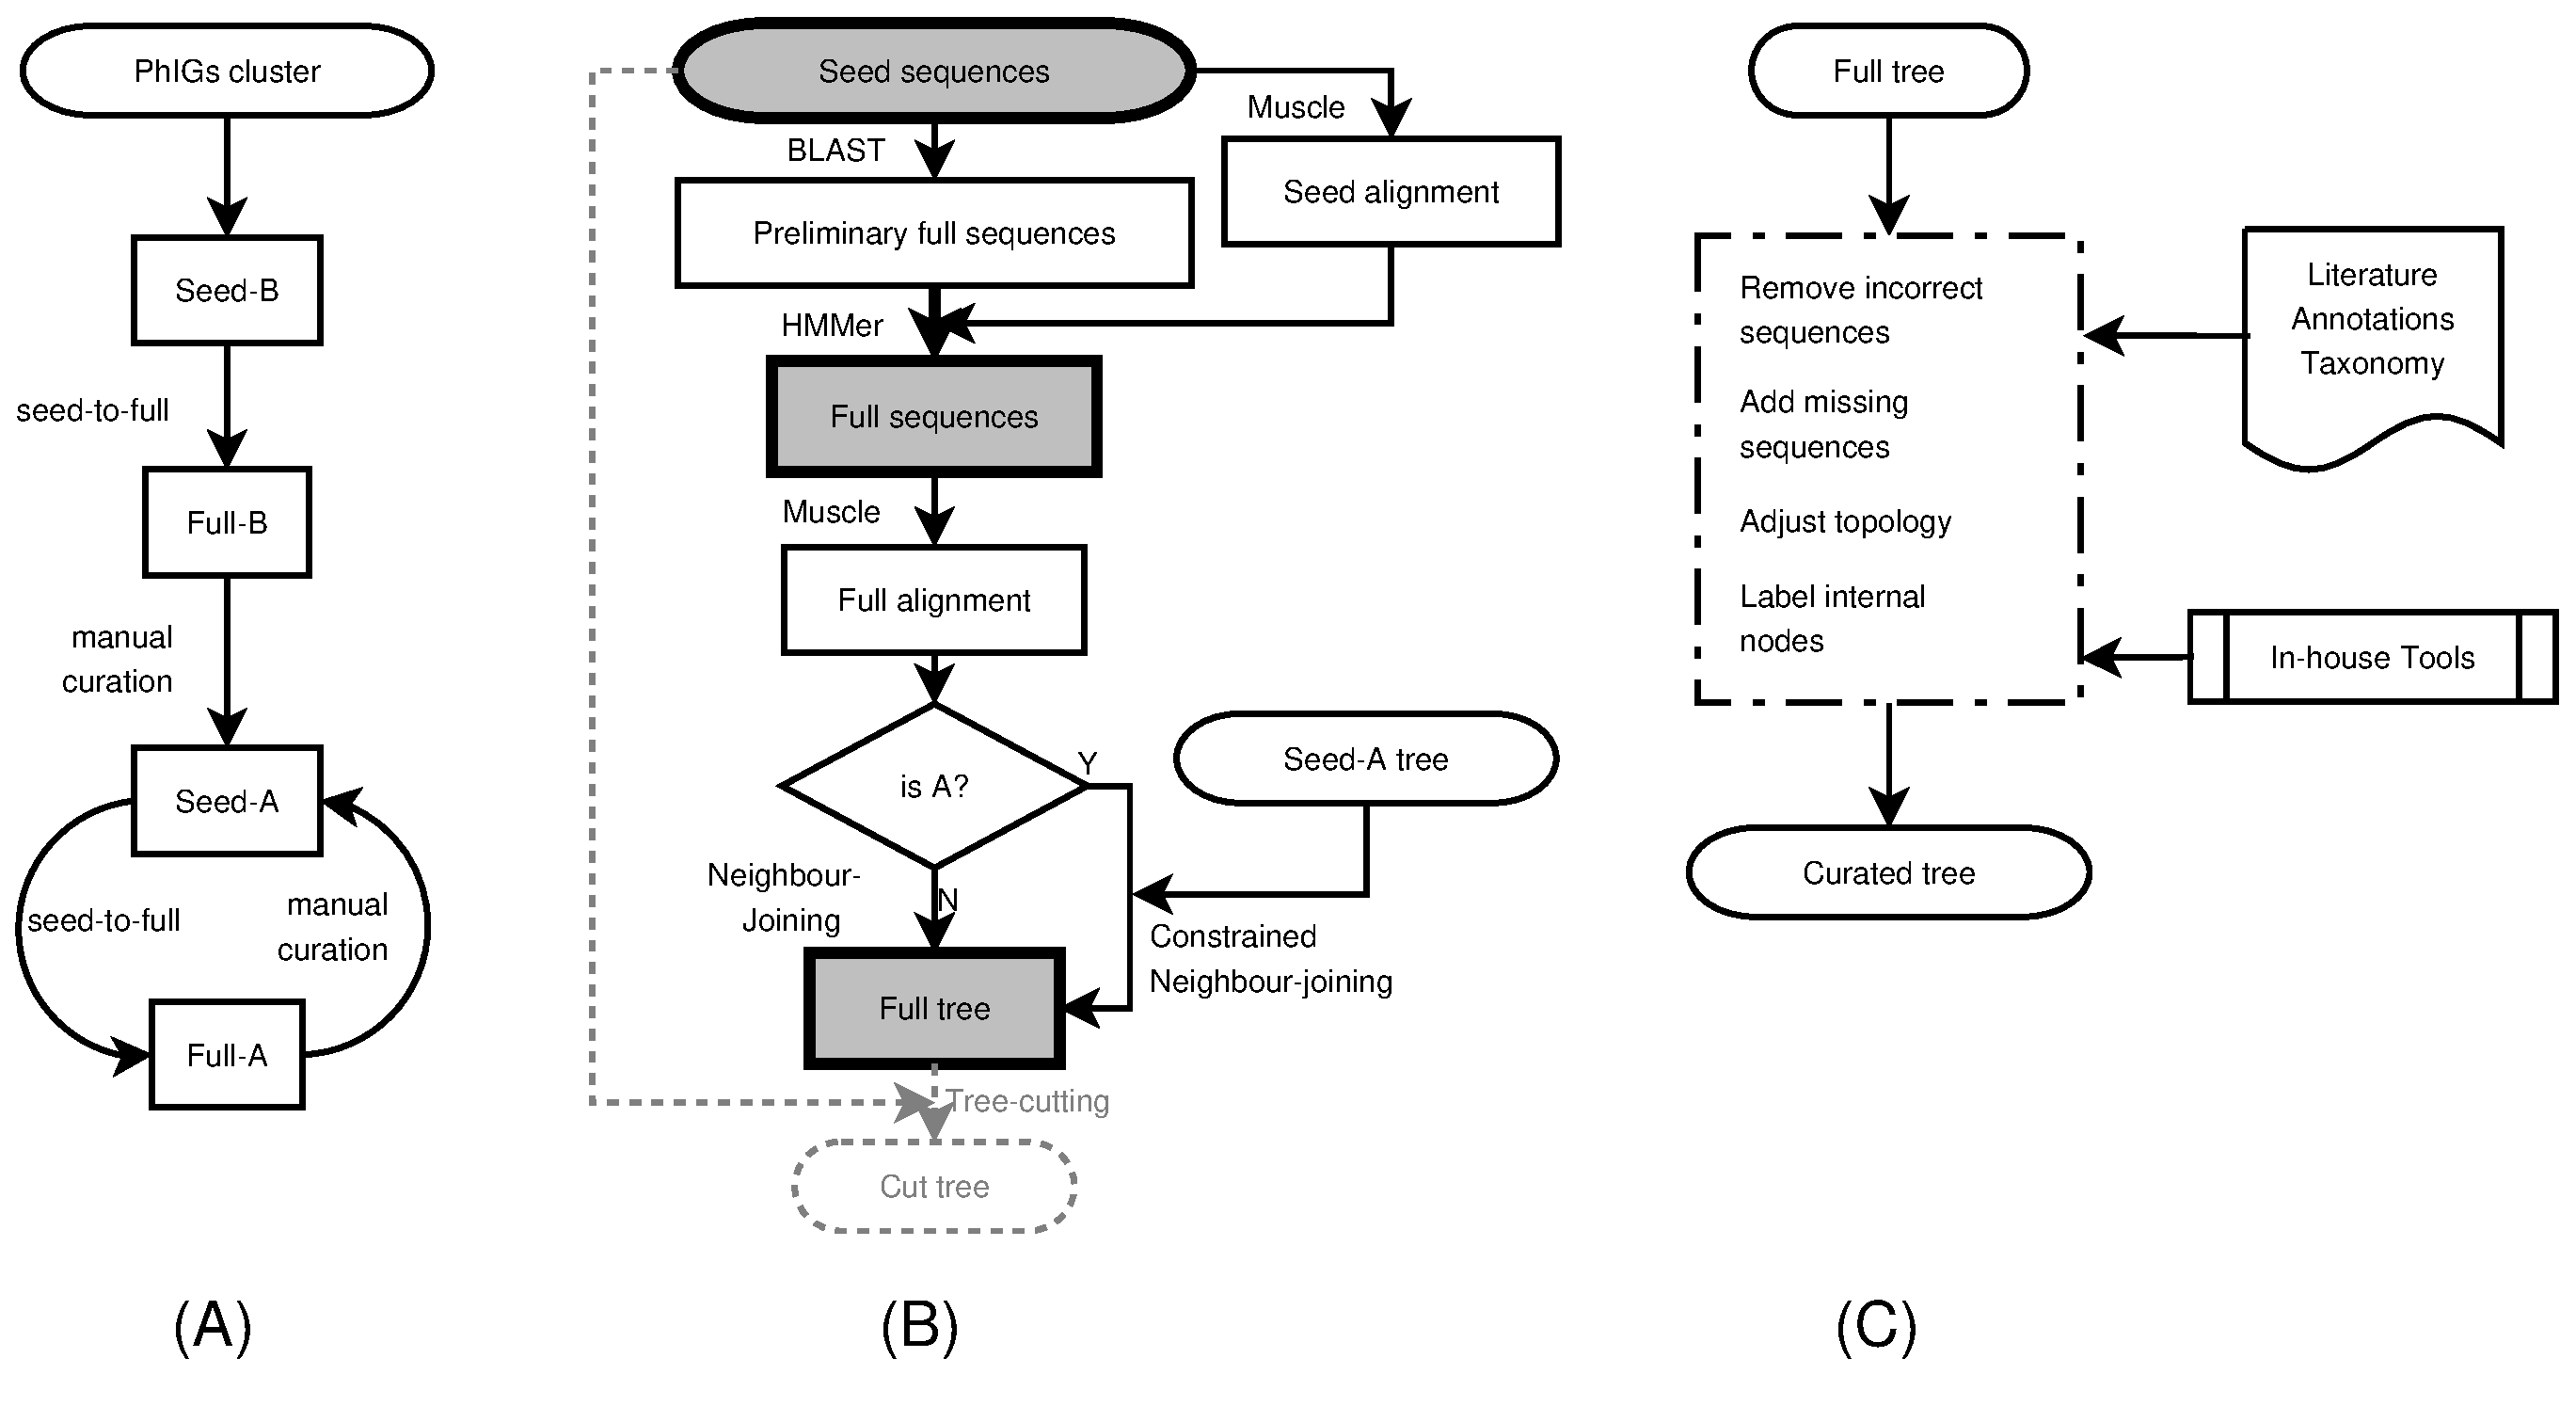
\includegraphics[width=\textwidth]{flowchart}
	\end{center}
}
\frame {
    \frametitle{Constructing TreeFam seeds}
    \begin{itemize}
    \item TreeFam-A: curated
    \item TreeFam-B: automatic
      \begin{itemize}
      \item TreeFam-1: PhIGs clusters
      \item TreeFam-2 and TreeFam-3: post-processed PhIGs clusters
      \item TreeFam-4: TreeFam-3 families
      \end{itemize}
    \end{itemize}
}
\frame {
	\frametitle{Seed-to-full expansion}
	\begin{itemize}
	\item BLAST seed sequences against the whole TreeFam sequence set (TFSEQ).
	\item Refine matched sequences with HMMER. HMM profiles are built from seed multialignment by MUSCLE.
	\item One {\it sequence} (or one transcript) is arbitrarily assigned to one family.
		One {\it gene} can be present in several.
	\end{itemize}
}
\frame {
	\frametitle{Reconstructing trees}
	\begin{itemize}
	\item Automatic full trees for TreeFam-B families
	\item Automatic `clean' trees for all families (tree merge)
	\item TreeFam-A full trees reconstructed by constrained neighbour-joining
	\item Branch lengths are estimated by ML algorithm combined with HKY model
	\end{itemize}
}
\section*{Acknowledgement}
\frame {
	\frametitle{Acknowledgement}
	\begin{itemize}
	\item Wang Jun (header of bioinformatics division of BGI)
	\item Richard Durbin (header of informatics division of Sanger)
	\item Zheng Wei-mou (supervisor)
	\item Li Ruiqiang, Liu Tao and Ruan Jue
	\item Avril Coghlan, Jean-Karim H\'{e}rich\'{e}, Lachlan James Coin, and Alan Moses (developers of Sanger)
    \item Albert and Abel (EBI Ensembl-compara group)
	\item all my friends in BGI and Aarhus University
	\end{itemize}
}
\frame {
	\begin{center}
	{\Huge Thank You!}
	\end{center}
}

\end{document}
